\section{Methods}

% Describe the architecture of your net, the training and validation process, regularisation methods you used, ...

% Beispiel des von uns gewünschten Pseudo-Code Layouts:

% \begin{algorithm}[H]
% \caption{Major Iteration: Bound-Constraint Lagrangian}
% \begin{algorithmic}
% \REQUIRE initial weights $ \boldsymbol w_{0} \in \mathbb{R}^{K} $, multipliers $\lambda^{0} $, inital value penality parameter $\gamma_{0}>0$ and given total convergence tolerances for $\eta_{*}$ and $\omega_{*}$
% % \ENSURE $y = x^n$
% \FOR{k = 1,2,\dots}

%     \STATE Using SQP finding an approximate solution for $w_{0}$ of the subproblem
%         \begin{equation*}
%           \left\| \boldsymbol w_{k}-P\left( \boldsymbol w_{k}-\nabla_{ \boldsymbol w} \mathcal{L}_{A}\left( \boldsymbol w_{k}, \lambda^{k} ; \gamma_{k}\right), l, u\right)\right\| \leq \omega_{k}
%         \end{equation*}

%     \IF{$\left\|c\left( \boldsymbol w_{k}\right)\right\|\leq\eta_{k}$}
%         \STATE{testing for convergence of given subproblem}

%         \IF{$\left\|c\left( \boldsymbol w_{*}\right)\right\|\leq \eta_{*} \land q_{k}( \boldsymbol w)\leq\omega_{*}$}
%             \STATE{\textbf{stop} approximate solution of $w_{k}$ found}

%         \ENDIF{ solution holds}
%             \STATE{Update the underlying multipliers \\
%             $\boldsymbol{\lambda}^{k+1}=\boldsymbol{\lambda}^{k}-\gamma_{k} c\left(x_{k}\right)$ \\
%             $\gamma_{k+1}=\gamma_{k}$
%             }

%         \ELSE
%             \STATE{If no valid solution was found and increase the penalties  \\
%             $\boldsymbol{\lambda}^{k+1}=\boldsymbol{\lambda}^{k}$ \\
%             $\gamma_{k+1}=100\gamma_{k}$}

%     \ENDIF


% \ENDFOR

% \end{algorithmic}
% \end{algorithm}

\subsection{Preprocessing}

This section covers all necessary preprocessing steps that build the foundation for all further modeling tasks.
Here, we mostly focus on feature \emph{engineering} by extracting information from the image and text data contained in the Airbnb Dataset.
However, feature \emph{selection} and transformations of the price variable turned out to be essential components of the preprocessing pipeline and are discussed in \Cref{appendix:feature-selection} and \Cref{appendix:price-distribution}.

In addition, some basic data cleaning steps at the very beginning were necessary.
These mostly consisted of converting data types, splitting text-based variables into more convenient numeric or boolean features and aggregating rare categories of categorical variables into one larger \emph{Other} group to stabilize estimation.
In order to later use the predictor variables as model inputs all features of categorical nature were transformed to Dummy variables whereas all numeric features were standardized.

Extending the original feature set with new informative covariates which are created from (combinations of) existing variables is a central aspect of every data analysis.
Besides many numeric features the Airbnb data contains \emph{images} as well as \emph{reviews} in raw text form.
These data types in particular require some extra care which will be the focus of this section.

\subsubsection{Image Processing and Modeling}

Besides the metric and text-based features the Airbnb Data contains \emph{images} of the listed apartments as well as of the corresponding hosts.
This section describes how we used these images (while focusing on the apartment pictures) for the purpose of price prediction.

The main idea was to build a Convolutional Neural Network (CNN) that predicts the price solely based on the image content itself and add these predictions as well as the number of available images for each listing to the main feature set.
Since there exist multiple images per apartment, the predictions were averaged afterwards within each group to obtain an output array of equal length to all remaining features.

Before the images can be used as model input they had to be \emph{scraped} from each listing's webpage.
Further, some basic transformations were necessary.
Details about these image proprocessing steps can be found in \Cref{appendix:images}.


\textbf{Image Modeling} \\
As mentioned above, we used a pretrained CNN for modeling.
Ideally, due to learning from a large collection of labeled images in a supervised setting, this model is able to extract meaningful features from our own much smaller input data out of the box.
As usual in \emph{transfer learning} the weights of the pretrained model are frozen and the output layer is replaced by a trainable custom layer specific to our needs.

One potential issue arises if the dataset used for pretraining differs from the new custom data:
If the pretrained network is very deep, the learned features before the final layer could be very specific to the Output Classes of \texttt{ImageNet} and not generalize well to our images.

There are multiple options to handle this scenario:
\begin{itemize}
  \item Out of the vast collection of freely available pretrained models, choose one that is comparably shallow.
        We chose \texttt{ResNet18} with roughly $11$ million parameters.
  \item Do not freeze the weights of the pretrained model completely, but rather fine tune them during training (i.e. modify \emph{all} weights by backpropagating through the entire network).
        We did not investigate this option further due to its high computational cost.
  \item Cut the pretrained model before the last layer with the hope that, at this point, very generic and widely applicable features of images are extracted.
        These features might in theory generalize better to our data.
        In practice, however, this option did not improve our results significantly.
\end{itemize}

It turned out that a \emph{single} custom layer, mapping from $512$ directly to a single neuron representing the scalar price prediction, was not expressive enough.
The performance improved by appending a (small) Fully Connected Network at the end instead containing three layers and \texttt{ReLU} activation functions.

To ensure that the chosen design is not majorly flawed, we constructed a separate much smaller CNN with only a handful of Convolutional Blocks as a benchmark model.
Although the performance differences were not as large as desired, the pretrained \texttt{ResNet} indeed indicated more promising results.


\textbf{Image Results} \\
Using only the content of the available images, the pretrained \texttt{ResNet18} achieved a Mean Absolute Error of $579$ NOK (approx. $58$ Euros) on the Validation Set.
In comparison, the \emph{Null Model} of always predicting the mean price achieved an MAE of $630$ NOK without a log-transformation of the price and a MAE of $569$ NOK with a log-transformation.
Thus, the raw predictive power of the images alone was very small.

However, the \emph{correlation} of the CNN predictions with the true price was $0.41$.
This indicates some limitations of the correlation as useful metric on the one hand but at least positive tendencies of the CNN predictions on the other hand.
In fact, the network struggled the most with capturing the wide \emph{range} of prices and almost always predicted values close to the center of the (log) price distribution.

Although the general idea of categorizing images into price ranges based on image features sounds very appealing, taking a look at the actual input images reveals how challenging this task actually is.
\Cref{fig:cnn-examples} in the Appendix displays a random collection of input images.
Considering the difficulty of the task it is actually highly doubtful that humans could provide much more accurate predictions.

\subsubsection{Reviews}

In order to extract the most important information from the reviews, we have performed the following analyses.

First, we used the \href{https://pypi.org/project/langdetect/}{langdetect} package to determine the language of each review.
With this information, we tried to get some insights about the internationality of the guests.
Since English and Norwegian are the most commonly used languages, we then created two so-called word clouds in these languages to visualize the most frequently used words in the reviews and to give us a short overview of the given ratings.
To just have the important words in this representation, a list of given stop words are used to extract them.
What is most striking in \Cref{fig:wordclouds} is that in both predominantly positive words are printed.
The largest printed and thus most frequently used words in English are \textit{apartment}, \textit{Oslo} and \textit{place} and further \textit{clean}, \textit{comfortable}, \textit{helpful} and \textit{easy}.
Also in the Norwegian plot there are mainly positive expressions like \textit{anbefale} (engl. \emph{recommend}), \textit{fin} (engl. \emph{fine}) and \textit{flott leilighet} (engl. \emph{great apartment}).

% insert Wordclouds english and norwegian side-by-side
\begin{figure}[t]
  \centering
  \begin{minipage}{6.7cm}
    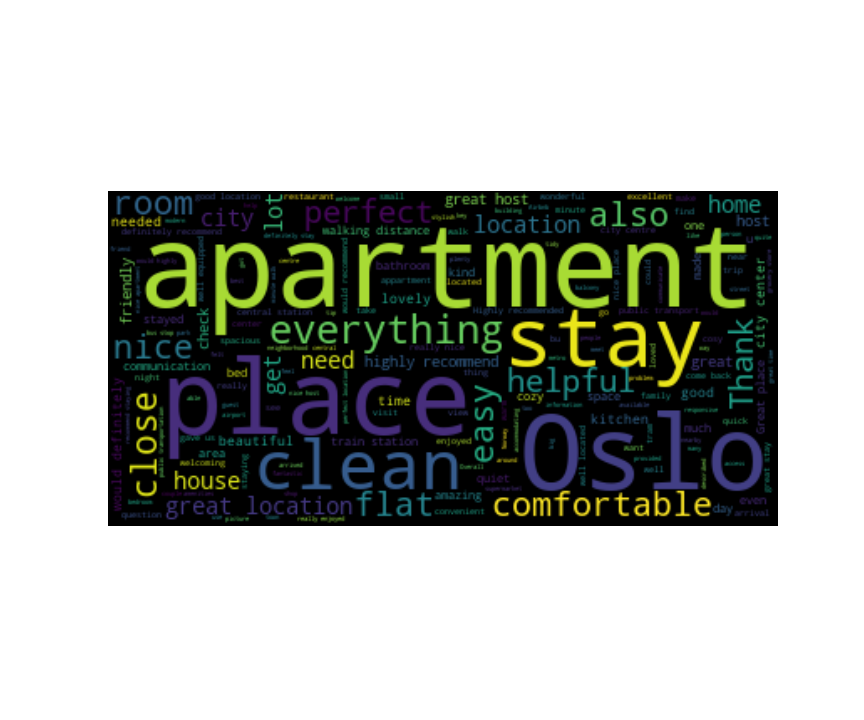
\includegraphics[width=\columnwidth]{wordcloud_eng.png}
  \end{minipage}
  \begin{minipage}{6.7cm}
    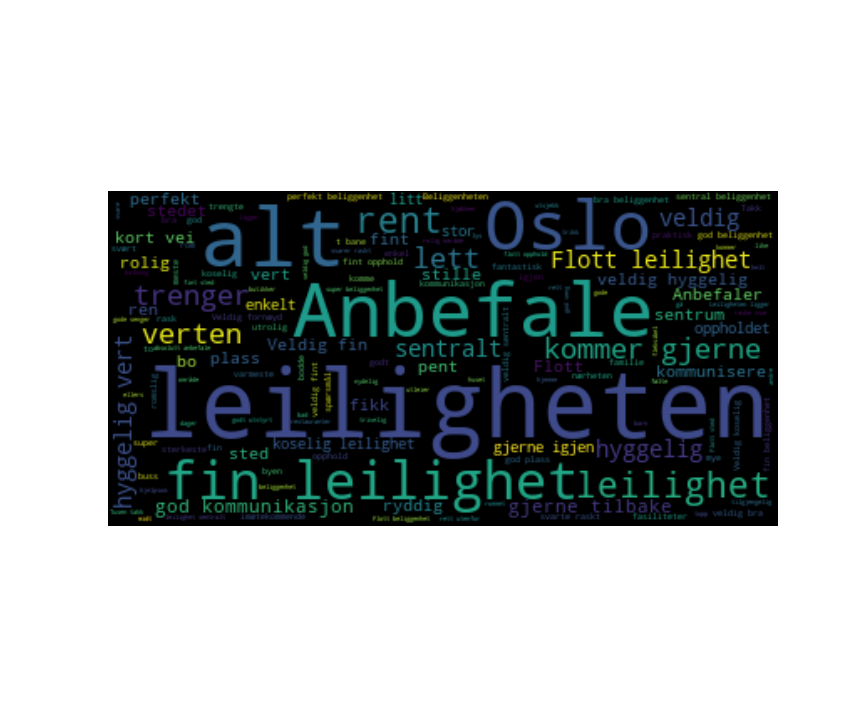
\includegraphics[width=\columnwidth]{wordcloud_nor.png}
  \end{minipage}
  \caption{Wordclouds in English and Norwegian}
  \label{fig:wordclouds}
\end{figure}

The results of the language detection are stored per \textit{listing\_id} in a new data frame called \textit{reviews\_features}.
This data frame contains the number of reviews per listing, the median length of a review, the number of different languages as well as a list of languages in which the reviews for that apartment were written.
The percentages of Norwegian and English reviews are also recorded for each listing id.
Finally, this data frame was added to the \textit{listings} data frame on which feature selection is performed later.
% COMMENT: (s. cite sentiment)

In addition, to obtain a more informed analysis of the reviews, we also performed a detailed sentiment analysis for each review.
Sentiment analysis is used to detect the underlying emotion of a text.
Therefore, it classifies the text as either positive or negative.

To do this, we used the \href{https://huggingface.co/transformers/v3.0.2/model_doc/distilbert.html}{transformers} package, more specifically we used the \href{https://huggingface.co/transformers/v3.0.2/main_classes/pipelines.html}{pipeline} function with the \texttt{task} argument set to \textit{sentiment-analysis}, which is used for classifying sequences according to positive or negative sentiments (s. documentation).
The used model is DistlBERT \citep{sanh2020}, a small, fast and light Transformer model, a distilled version of BERT \citep{devlin2019} algorithm, which achieves significantly faster results.

Finally, we used the sentiment analysis to determine the ratio of negative reviews to the total number of reviews per listings id, which is also added to the \textit{reviews\_feature} data frame.

% TODO: Include in Bibliography
%Analysis: https://towardsdatascience.com/a-beginners-guide-to-sentiment-analysis-in-python-95e354ea84f6

\subsection{Models}

This section describes the statistical models that we used to predict apartment prices based on their feature set.
The goal is to construct different models of varying complexity and compare both their in-sample and their out-of-sample performance on the Airbnb data.

At this point in the data pipeline all preprocessing steps are completed such that all covariates have the correct data type to be used by the models.
Whereas the selected classical Machine Learning models described in \Cref{classical-models} use input features as \texttt{numpy} arrays, the Neural Network in \Cref{neural-network} first converts them to \emph{Tensors}, the canonical data type across all popular Deep Learning Frameworks.

\subsubsection{Classical Models} \label{classical-models}

When attacking the prediction task directly with a Neural Network, there are two questions that we cannot answer:
%%%
\begin{enumerate}
  \item How do we know if a performance metric is \emph{good}?
  \item Is fitting a Neural Network appropriate in the first place?
        Maybe we can get away with a much simpler, more interpretable and, thus, preferable model?
\end{enumerate}
%%%
In order to get some insights, we selected four classical Machine Learning models of varying complexity from the \texttt{scikit-learn} library \citep{pedregosa2011} to serve as benchmark models for our custom Neural Net.
These include:
%%%
\begin{itemize}
  \item \href{https://scikit-learn.org/stable/modules/generated/sklearn.linear_model.LinearRegression.html}{Linear Regression}: simple, well understood in terms of underlying theory and highly interpretable.
  \item \href{https://scikit-learn.org/stable/modules/generated/sklearn.linear_model.Ridge.html}{Ridge Regression}: still very interpretable with a closed form analytical solution, adds one hyperparameter to the equation.
  \item \href{https://scikit-learn.org/stable/modules/generated/sklearn.ensemble.RandomForestRegressor.html}{Random Forest}: very flexible model with many hyperparameters determining e.g. the number of regression trees and the tree depth.
        Can be applied to many contexts and often works 'out of the box'.
  \item \href{https://scikit-learn.org/stable/modules/generated/sklearn.ensemble.HistGradientBoostingRegressor.html}{Histogram-Based Gradient Boosting}: modern and fast tree-based gradient boosting algorithm.
        Comes with a large number of tunable hyperparameters, some of them similar to the Random Forest parameters, some of them more specific to the \emph{Boosting} instead of the \emph{Bagging} approach such as the learning rate.
        Similar to the very popular \href{https://xgboost.readthedocs.io/en/stable/}{XGBoost} \citep{chen2016} and \href{https://lightgbm.readthedocs.io/en/latest/}{LightGBM} \citep{ke2017} implementations that regularly outperform deep Neural Networks in Kaggle competitions on tabular data.
\end{itemize}
%%%

All models were fitted with \emph{Cross Validation}.
Except for the Linear Regression this included (extensive) \emph{Hyperparameter Tuning}.
Since the parameter space for both of the tree-based models is very high-dimensional we used a \emph{Randomized Search} algorithm \citep{bergstra2012} rather than the more common \emph{Grid Search} approach.
This allows for greater variation along more 'important' dimensions while still keeping the computation time feasible.


\subsubsection{Neural Network} \label{neural-network}

In concurrence with the Seminar's topic the focus of our project is centered around constructing a custom Neural Network that is trained in a supervised setting and learns to map feature combinations to price predictions for the Airbnb data set.
The following section highlights the key components of the model's architecture.
A brief overview of additional (hyper-)parameters that were of minor importance can be found in \Cref{appendix:hyperparameters}.

The network's design is restricted by two factors:
%%%
\begin{enumerate}
  \item The number of input features in the \emph{first} layer has to equal the number of features used for prediction.
  \item The number of output features in the \emph{last} layer is fixed to $1$ since the network directly predicts the price as a scalar quantity.
\end{enumerate}
%%%
All intermediary layers and thus both the \emph{width} and the \emph{depth} of the network are free to choose.
After experimenting with many different configurations, mostly inspired by empirical findings in the literature, we finally settled with a fairly simple \emph{block structure}.

Starting from roughly $60$ input features, the network width is first blown up to $256$ features before steadily decreasing it again to a single output neuron in the final layer.
More precisely, the architecture consists of $6$ intermediary \textbf{blocks} with $64$, $128$, $256$, $128$, $64$ and $8$ output features in addition to the linear input and output layers.

%%%
\begin{figure}[t]
  \centering
  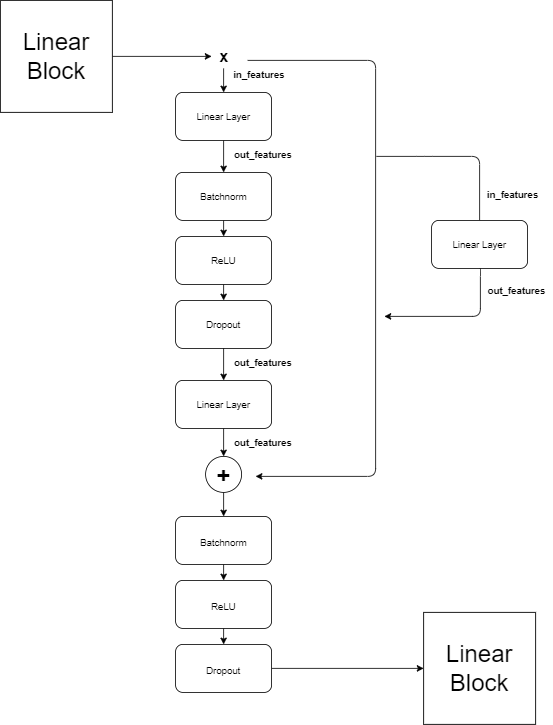
\includegraphics[width=0.7\textwidth]{mlp_architecture.png}
  \caption{Architecture of each Block in the Fully Connected Neural Network}
  \label{fig:linear-block}
\end{figure}
%%%

The structure of each so-called \texttt{Linear Block} is displayed in \Cref{fig:linear-block}.
We now explain the reasoning behind including or excluding elements in this configuration.

\textbf{Linear Layer} \\
Each \texttt{Linear Block} is based on a four-element cycle that is repeated twice.
Each cycle starts with a Fully-Connected Layer containing the majority of trainable weights in the network.
The first linear layer determines the output dimension of this block, in our case mostly doubling or halving the number of input features.
Since both linear layers are immediately followed by a \texttt{Batchnorm} Layer, the additional \texttt{Bias} term is redundant and thus omitted.

\textbf{Batchnorm} \\
\texttt{Batchnorm} Layers \citep{ioffe2015} often lead to a more well-behaved training process.
By means of first standardizing the activations within each minibatch and rescaling them afterwards, the network \emph{learns} a convenient magnitude of the activations.
This tends to be particularly effective for \emph{saturating} activation functions such as \texttt{sigmoid} or \texttt{tanh} activations, positive effects for training, however, have also been observed for the \texttt{ReLU} activation function, which is used in our design.
Of all individual components of the \texttt{Linear Block} structure, Batchnorm was the least important and provided only marginal benefits.

\textbf{ReLU} \\
Out of the numerous options for including nonlinearities into the network and thus expanding the function space that the network is able to learn, we settled for the default choice of the \emph{Rectified Linear Unit} activation.
While briefly experimenting with the related \texttt{Leaky ReLU} and \texttt{Exponential ReLU}, the differences were insignificant and could be easily attributed to other factors such as random weight initialization.

\textbf{Dropout} \\
The \texttt{Dropout} Layer \citep{srivastava2014} at the end of each cycle turned out to be the single most impactful factor for the network's \emph{generalization} ability.
In fact, due to the different behaviour of dropout during training and inference, we could directly control the relative performance on training and validation set by varying the dropout probability $p$.

More specifically, the network overfitted drastically by setting $p$ to zero.
This actually provided the valuable insight that the current function class is flexible enough to model the task at hand properly.
Thus, there was no need to artificially expand the network size beyond the current quite compact architecture with roughly $280.000$ trainable parameters, saving computation time as a nice side-effect.

\Cref{fig:dropout} in the Appendix displays the shift in performance metrics on training and validation set when steadily increasing the dropout probability $p$.
While not beneficial for overall performance, dropout delivers a leverage to make the model perform much better on out-of-sample data compared to the dataset that it was actually trained on.

This behaviour can be explained by the \emph{ensemble} interpretation of dropout \citep{goodfellow2016}:
In each epoch, a different subset of neurons is excluded to contribute to training and thus a distinct subset model, nested in the full model, is responsible for the prediction output.
If the dropout probability is extremely high, these subset models are simply too different from each other and do \emph{not agree} on a common range of sensible prediction values.

In contrast, during inference (and possible deployment of the model), any randomness should be avoided and the network may use all of its neurons.
Although there is no influence on the model \emph{weights} in this stage, the model pools all subset models together and \emph{averages out} the diverging effects of each component, ultimately resulting in better performance metrics.

\textbf{Residual Connections} \\
One special feature of the \texttt{Linear Block} architecture in \Cref{fig:linear-block} is the \emph{Residual Connection} which adds the block input to the output of the second linear layer within each block.
This component was originally implemented having a fairly deep network in mind since \emph{Residual Blocks} introduced by the famous \texttt{ResNet} architecture \citep{he2015} are a very popular tool for stable gradient flow by preventing the issue of vanishing gradients.

As mentioned above the actual depth of the final model turned out to be limited.
Therefore we decided to enable inclusion and exclusion of skip-connections in the network by a \texttt{boolean} parameter allowing for easy comparisons between the model designs.
Although the residual component did not have a major impact on performance, it was slightly beneficial in most settings such that there was no reason to remove it from the architecture.

There are two aspects worth mentioning about the residual connection in \Cref{fig:linear-block}:
%%%
\begin{enumerate}
  \item The addition of the input with the output of the second linear layer is performed \textbf{before} the final \texttt{Batchnorm} and \texttt{ReLU} layers of this block.
        This guarantees a nonnegative input in the expected range for the next \texttt{Linear Block} since the raw outputs of a fully connected layer are (in theory) unbounded.

  \item One caveat of the residual architecture is to ensure that at addition time all contributing terms share the same dimensions.
        In case of a fully connected layer dealing with two-dimensional tensors, this amounts to an equal number of features in the second dimension.
        As illustrated by the annotations in \Cref{fig:linear-block}, this restriction requires an extra step if the number of input features is different from the number of output features in this particular block.
        In our case the dimnesions adjustment is performed by an additional linear layer exclusively for the block input $x$.
\end{enumerate}
%%%

